% 2. Indledning
\chapter{Indledning}

I det moderne hjem er der ofte en skiftende brug af hjemmets største fællesrum, nemlig stuen. Stuen skal kunne tilpasses så den kan lægge rum til alle beboernes sociale behov. Dette kan være alt fra aftensmaden hvor familien er samlet rundt om bordet, særlige brætspilsaftener eller nytårsfest hvor der skal danses. En af problemstillingerne ved at tilpasse et rum til så forskellige begivenheder er belysningen.

Produktet L.A.M.P. (Light And Movement Project) er den dynamiske lampe med talrige kombinationsmuligheder for at opfylde belysningsbehovet i den meget alsidige stue. 

L.A.M.P skal kunne flytte belysningen til et hvilket som helst sted i rummet. Det skal kunne ændre belysningen efter behov. Det skal kunne detektere bevægelse i rummet og efter brugerens valg reagere herpå. Det skal kunne indstille lampens lys-output i forhold til allerede eksisterende værdier af lys i rummet f.eks. ved morgentimerne under sommer-/vintertid.  

Når disse krav er opfyldt, kan L.A.M.P. installeres i mere end kun private hjem. Sygehusenes operationsstuer er særligt udfordret i forhold til at få den optimale belysning, hvortil denne lampe ville kunne give et nyt perspektiv på en mulig løsning. 

L.A.M.P. er tiltænkt til installation under loftet i rektangulære rum. Der monteres to skinner på langs af rummet under loftet. På disse skinner placeres der en vogn der dermed går på tværs af rummet. Denne vogn har motorer i begge ender, der kan kører på de skinner der går på langs af rummet. Dette gør at vognen kan kører på langs af rummet, altså rummets X-akse. På den vogn der her er placeret, placeres der endnu en vogn. Denne kan kører på tværs af rummet, altså rummets Y-akse. I bunden af denne vogn er der monteret et hejs, som kan hæve og sænke lampen op og ned og dermed bevæge lampen på rummets Z-akse. Hermed kan lampen bevæge sig frem, tilbage, sidelæns, op og ned i rummet og kan dermed flyttes til alle positioner i rummet. Se figur \ref{fig:3D_Koncept}

\begin{figure}[H] \centering
    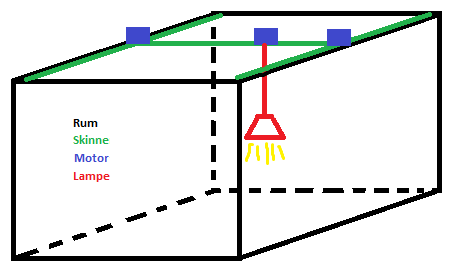
\includegraphics[width=\textwidth]{Filer/3D_Koncept.png}
    \caption{3D koncept tegning}
    \label{fig:3D_Koncept}
\end{figure}

Produktet der gennem denne rapport er fremstillet, er bygget som en prototype. Dette er grundet at det skal kunne tilpasses et hvert lokale, og dermed ikke kunne bygges i systemets endelige form. Yderligere skal systemet kunne præsenteres og det er dermed en nødvendighed at kunne flytte det.  	

For at gennemføre projektet bedst muligt blev det opdelt i områder. Hvert gruppemedlem blev tildelt et arbejdsområde, enten enkeltvis eller i par, som skulle arbejdes med og løses. Fordelingen af gruppemedlemmer og arbejdsområder blev aftalt som følger: 

\begin{table}[H] \centering
\begin{tabular}{|l|p{10cm}|}
	\hline
	\textbf{Jeppe}		
	    & Kommunikationen mellem PSoC’s via PSoC-Master
	\\ \hline
	\textbf{Victor} 		
	    & GUI på Devkit8000
	\\ \hline
	\textbf{Kimmie og Simon} 		
	    & Lysniveau-, bevægelse-, afstands-sensor og lys, samt styring af disse på PSoC-Sensor
	\\ \hline
	\textbf{Kasper og Casper} 	
	    & Bevægelse i X- og Y-retning, detektering af ende-position samt styring af dette på PSoC-XY
	\\ \hline
	\textbf{Andreas} 			
	    & Bevægelse i Z-retning, detektering af øverste ende-position samt styring af dette på PSoC-Z
	\\ \hline
\end{tabular}
\end{table}